\documentclass[a4paper, ngerman]{scrartcl}
\usepackage[utf8]{inputenc}
\usepackage[T1]{fontenc}
\usepackage{babel, lmodern, amsmath, amsfonts, graphicx, amssymb, mathrsfs, xcolor, pgfplots}
\pgfplotsset{width=10cm, compat=1.18}
\usetikzlibrary{patterns}

\newcommand{\oversetcustom}[2]{\overset{\scalebox{1.3}{\textcolor{red}{#1}}}{#2}}

\begin{document}
	\title{Lösungen der Übungsaufgaben Analysis 2 für den 17.10.24}
	\author{Emanuel Schäffer}
	\maketitle
	
	\section*{Aufgabe 1}
	\subsubsection*{Nullstellen bestimmen}
	\begin{flalign*}
		f(x) &= \frac{2x+1}{2x^2+2x-1}\\
		x_{1,2} &= \frac{-2\pm\sqrt{2^2-4\cdot2\cdot(-1)}}{2\cdot2} \\
		x_{1,2} &= \frac{-2\pm2\sqrt{3}}{4} \\
		x_{1,2} &= \frac{-\not{2}\pm\not{2}\sqrt{3}}{\not{4} \quad 2} \\
		\Rightarrow x_1 = -\frac{1}{2}(1-\sqrt{3}) & \qquad x_2 = -\frac{1}{2}(1+\sqrt{3}) 
	\end{flalign*}
	
	\subsubsection*{Produktform}
	\begin{equation*}
		(x + \frac{1}{2}(1-\sqrt{3}))(x + \frac{1}{2}(1+\sqrt{3})) \oversetcustom{?}{=} 2x^2+2x-1 
	\end{equation*}

	\subsubsection*{Partialbruch}
	\begin{equation*}
		\frac{\alpha}{x+\frac{1}{2}(1-\sqrt{3})} + \frac{\beta}{x+\frac{1}{2}(1+\sqrt{3})} 
	\end{equation*}

	\begin{flalign*}
		\alpha(x+\frac{1}{2}(1+\sqrt{3})) &+ \beta(x+\frac{1}{2}(1-\sqrt{3})) \oversetcustom{!}{=} x + \frac{1}{2}\\
		\alpha x + \alpha\frac{1}{2}(1 + \textcolor{red}{\underline{\sqrt{3}}}) &+ \beta x +  \beta \frac{1}{2}(1 - \textcolor{red}{\underline{\sqrt{3}}}) 
	\end{flalign*}
	\qquad \textcolor{red}{$\rightarrow$ Keine irrationalen Zahlen im Zähler, daher $\alpha = \beta$}
	$$ \alpha x + \beta x = x  \quad \Rightarrow \alpha = \beta = \frac{1}{2}$$ 

	\begin{flalign*}
		\Rightarrow \frac{\frac{1}{2}}{x + \frac{1}{2}(1 - \sqrt{3})} &+ \frac{\frac{1}{2}}{x + \frac{1}{2}(1 + \sqrt{3})}\\
		\int \frac{2x + 1}{2x^2 + 2x - 1} = \int \frac{\frac{1}{2}}{x + \frac{1}{2}(1 - \sqrt{3})} &+ \int \frac{\frac{1}{2}}{x + \frac{1}{2}(1 + \sqrt{3})}\\
		= \frac{1}{2}\ln(x + \frac{1}{2}(1 - \sqrt{3}) &+ \ln(x + \frac{1}{2}(1 + \sqrt{3}))\\\\
		=\ln(x^2 + x -\frac{1}{2})\\
		=\ln(2x^2 + 2x -1)
	\end{flalign*}

	\section*{Aufgabe 2}
	
	\[
	\text{Da } \displaystyle \int_{1}^{\infty} \frac{1}{x^2} \, dx = 1 \text{ und Fläche von } x=1-2 \text{ von } \frac{1}{x^2} > 0 \Rightarrow \displaystyle \sum_{i=2}^{\infty} \frac{1}{i^2} < 1
	\]
	
	\begin{figure}[htbp]
		\centering
		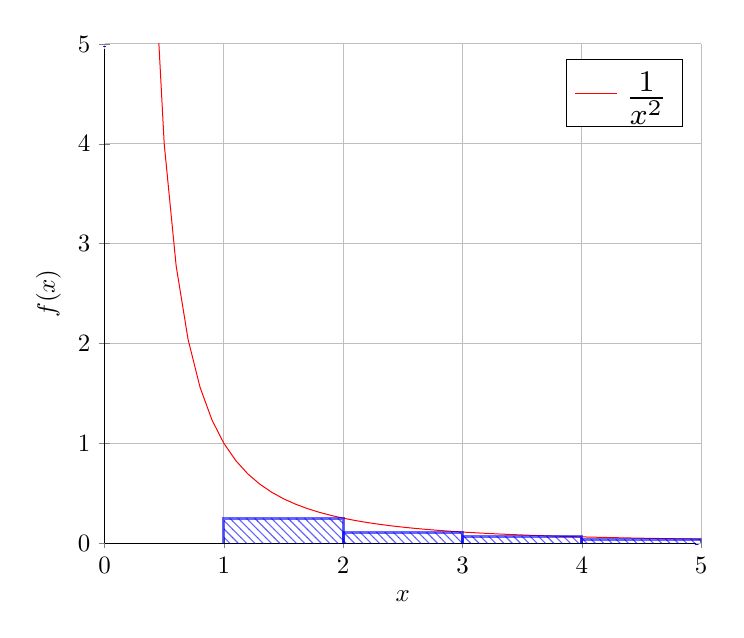
\begin{tikzpicture}[scale=0.9]
			\begin{axis}[
				axis lines=left,
				xlabel=$x$,
				ylabel=$f(x)$,
				xmin=0, xmax=5,
				ymin=0, ymax=5,
				grid=major,
				legend pos=north east,
				legend style={font=\large, scale=1.5, nodes={scale=1.5}},
				pattern color=blue, 
				pattern=horizontal lines
				]
				\addplot[
				domain=0.1:5,
				samples=50,
				color=red
				] {1/x^2};
				\addlegendentry{$\frac{1}{x^2}$}
				
				\draw[blue, very thick, opacity=0.6] (axis cs: 1,0) -- (axis cs: 1,{1/2^2}) -- (axis cs: 2,{1/2^2}) -- (axis cs: 2,0);
				\draw[blue, very thick, opacity=0.6] (axis cs: 2,0) -- (axis cs: 2,{1/3^2}) -- (axis cs: 3,{1/3^2}) -- (axis cs: 3,0);
				\draw[blue, very thick, opacity=0.6] (axis cs: 3,0) -- (axis cs: 3,{1/4^2}) -- (axis cs: 4,{1/4^2}) -- (axis cs: 4,0);
				\draw[blue, very thick, opacity=0.6] (axis cs: 4,0) -- (axis cs: 4,{1/5^2}) -- (axis cs: 5,{1/5^2}) -- (axis cs: 5,0);
				\fill[pattern=north west lines, pattern color=blue, opacity=0.6] 
				(axis cs: 1,0) rectangle (axis cs: 2,{1/2^2});
				\fill[pattern=north west lines, pattern color=blue, opacity=0.6] 
				(axis cs: 2,0) rectangle (axis cs: 3,{1/3^2});
				\fill[pattern=north west lines, pattern color=blue, opacity=0.6] 
				(axis cs: 3,0) rectangle (axis cs: 4,{1/4^2});
				\fill[pattern=north west lines, pattern color=blue, opacity=0.6] 
				(axis cs: 4,0) rectangle (axis cs: 5,{1/5^2});
			\end{axis}
		\end{tikzpicture}
	\end{figure}
	
	
	\section*{Aufgabe 3}
	$\rightarrow$ Siehe Musterlösung
	
	\nopagebreak
	
	\section*{Aufgabe 4}
	$\rightarrow$ Siehe Musterlösung, Script Seite 9.
	
\end{document}